\begin{frame}
  \begin{center}
    {\huge A* Sampling
    } \\
    Maddison,Tarlow,Minka
  \end{center}
\end{frame}

%% \begin{frame}{Premise of the Paper}
%%   %% what is the paper trying to solve
%% \end{frame}


%%%%%%%%%%%%%%%%%%%%%%%%%%%%%%%%%%%%%%%%%%%%%%%%%%
\begin{frame}{Partition Function Woes}
  Gibbs Distribution
  \begin{align*}
    \Pr(\x;\theta) =\frac{\exp(\theta^T\phi(\x))}{Z} \tag{$Z=\sum_{\x} \theta^T\phi(\x)$ is partition function}
  \end{align*}
  ML parameter estimation,
  \begin{align*}
    - \nabla_\theta \log LLH = \E_{\Pr(x;\theta)}\left[\phi(\x)\right] - \frac{1}{T} \sum_i\phi(x_i)
  \end{align*}
  Computing $\E_{\Pr(x;\theta)}$ is not usually tractable (Sampling from posterior is hard).
  Resort to approximations - MCMC, Contrastive Divergence etc.
\end{frame}

%%%%%%%%%%%%%%%%%%%%%%%%%%%%%%%%%%%%%%%%%%%%%%%%%%
\begin{frame}{Gumbel Distribution}
  \begin{align*}
    & Gumbel(m) = \text{gumbel with location parameter $m$}\\
    %% & CDF(x;\mu) = \exp \left(-\exp\left(-x+\mu\right)\right) \\
    & F_m(g) = \Pr(G\le g) = \exp(-\exp(-g+m)) \tag{CDF for $Gumbel(m)$}\\
    & Mean = \mu+\gamma \tag{a fixed offset away from location parameter} \\
    & Variance = \frac{\pi^2}{6}
  \end{align*}
\end{frame}

%%%%%%%%%%%%%%%%%%%%%%%%%%%%%%%%%%%%%%%%%%%%%%%%%%
\begin{frame}{Key Properties}
  For $G(i) \sim Gumbel(0)$,
  \begin{align*}
    & \argmax_i{G(i)+\phi(i)} \sim \frac{\exp(\phi(x))}{Z} \\
    & \max_i{G(i)+\phi(i)} \sim Gumbel(\log Z) \tag{Max-Stability}
    %% proof in \cite{hazan}
  \end{align*}
\end{frame}

%%%%%%%%%%%%%%%%%%%%%%%%%%%%%%%%%%%%%%%%%%%%%%%%%%
\begin{frame}{Gumbel-Max Trick (Discrete Case)}
  Suppose you have a discrete distribution specified by un-normalized log probabilities $\{\phi(i)\}_{i=1}^{k}$, i.e.,
  \begin{align}
    \Pr(x_i) = \frac{\exp\phi(i)}{\sum_j\exp\phi(j)} \label{eq:gibbs}
  \end{align}
  We can draw samples $x_i \sim \Pr$ from this distribution using the following procedure.
  \begin{align*}
    & \text{Sample} \qquad G(i) \sim Gumbel(0) \text{ for } i=1..k\\
    & \text{then} \qquad x_i \sim \argmax_i \{G(i) +\phi(i)\} \tag{the argmax of the perturbed probabilities is distributed as eq.\ref{eq:gibbs} above}
  \end{align*}
  No need to compute the partition function, as long as you can compute the (perturbed) argmax!
  Note that the samples are exact. (No approximations!) (examples when things are approximations)
\end{frame}

%%%%%%%%%%%%%%%%%%%%%%%%%%%%%%%%%%%%%%%%%%%%%%%%%%
\begin{frame}{Is There A Gumbel Max Trick for Continuous Distributions?}
  This paper --- Yes!
\end{frame}

%%%%%%%%%%%%%%%%%%%%%%%%%%%%%%%%%%%%%%%%%%%%%%%%%%
\begin{frame}{Gumbel and the Partition Function}
  
\end{frame}

%%%%%%%%%%%%%%%%%%%%%%%%%%%%%%%%%%%%%%%%%%%%%%%%%%
\begin{frame}{Gumbel Process}
  %% just put image
\end{frame}

%%%%%%%%%%%%%%%%%%%%%%%%%%%%%%%%%%%%%%%%%%%%%%%%%%
\begin{frame}{High Dimensional Sampling is Exponential}

\end{frame}

%%%%%%%%%%%%%%%%%%%%%%%%%%%%%%%%%%%%%%%%%%%%%%%%%%
\begin{frame}{Top-Down Construction of Gumbel Process}
  Assume log Z is computable for now.
\end{frame}

%%%%%%%%%%%%%%%%%%%%%%%%%%%%%%%%%%%%%%%%%%%%%%%%%%
\begin{frame}{Main Idea}
  \emph{We can transform a Gumbel process into another by adding the difference of their log densities.} \\
  log Prior + log LLH = log Posterior
  Suppose
  So if I can easily draw samples from the prior and I have a way to compute the bound on the log-likelihood, then I can use Gumbel.
\end{frame}

\begin{frame}{Main Idea}
  \centering
  \begin{tikzpicture}[scale=0.8]
    %% \draw[step=0.5,gray] (-5,-5) grid (5,5);
    \draw[ultra thick,gray] plot[smooth] coordinates {(-6,0)(-5,0)(-3,3) (0,-1) (3,3) (5,0)};
    \node (ox) at (-4,-1) {o(x)};

    %% \begin{axis}[height=10cm,width=10cm]
    %%   \addplot[ultra thick,gray,smooth] coordinates {
    %%     (-6,0)(-5,0)(-3,3) (0,-1) (3,3) (5,0)}
    %%   node [pos=0.9,below left] {o(x)};
    %% \end{axis}
    
    \only<2>{
      \path[draw,dotted,blue,very thick] (-5,5) -- (5,5);
    }
    %% \addplot+[ycomb,black,thick] {1};
    %% \node[above] (g1) at (0,4) {};

    \onslide<2->{
      \path[draw,red,thick] (0,-1) -- (0,4) circle (1.5pt);
      \node[above] at (0,4.25) {$g_1+o(x_1)$};
    }
    
    \only<2,3>{
      \path[draw,green,dotted,very thick] (-5,4) -- (5,4);
    }
    
    \onslide<3->{
      \path[draw,red,thick] (-3,3) -- (-3,2) circle (1.5pt);
      \node[below] at (-3,1.5) {$g_2+o(x_2)$};
    }

    \only<3,4,5>{
      \path[draw,dotted,blue,very thick] (-5,3.5) -- (0,3.5);
    }
    
    \onslide<4->{
      \path[draw,red,thick] (3,3) -- (3,4.5) circle (1.5pt);
      \node[below] at (3,5.25) {$g_3+o(x_3)$};
    }
    \only<3->{
      \path[draw,dotted,blue,very thick] (0,5) -- (5,5);
    }
    \only<4->{
      \path[draw,green,dotted,very thick] (-5,4.5) -- (5,4.5);
    }
  \end{tikzpicture}  
\end{frame}

\begin{frame}
  But
\end{frame}
